
%(BEGIN_QUESTION)
% Copyright 2006, Tony R. Kuphaldt, released under the Creative Commons Attribution License (v 1.0)
% This means you may do almost anything with this work of mine, so long as you give me proper credit

Identify the purpose of the pushbutton switch in this integrator circuit:

$$\includegraphics[width=15.5cm]{i01582x01.eps}$$

Then, give a practical example of this switch's use, in an application where the integrator circuit is integrating some real-life measurement signal. 

\underbar{file i01582}
%(END_QUESTION)





%(BEGIN_ANSWER)

If this integrator were used to ``totalize'' the number of gallons of liquid stored in a vessel from a flowmeter signal, the switch could be used to reset the totalized quantity to zero after each time the vessel is emptied.

%(END_ANSWER)





%(BEGIN_NOTES)

The switch serves the same purpose as a ``trip odometer'' reset button in an automobile.

%INDEX% Electronics review: integrator circuit

%(END_NOTES)


